\documentclass[12pt]{article}
\usepackage[left=2cm, top=2cm, right=2cm, bottom=2cm]{geometry}
\usepackage[utf8]{inputenc}
\usepackage[T1]{fontenc}
\usepackage[french]{babel}
\usepackage{graphicx}
\usepackage{graphics}
\usepackage{amsmath}
\usepackage{tikz}
\usepackage{graphicx}
\usepackage{xcolor}
\usepackage{parskip}
\usepackage{physics}
\usepackage{gensymb}

\title{\textbf{Instrumentation} \\ TP 2: Caractérisation d'un capteur de température}
\author{MENARD Alexandre \\ VIEILLEDENT Florent \\ RANCHY Nilo}

\setlength{\parindent}{1cm}

\begin{document}
\maketitle

\section*{Introduction}
Dans ce travail pratique, on étudie les caractéristiques d'un capteur de température PT100. Le capteur est composé notamment d'une couche de platine dont la résistance varie en fonction de la température. Le capteur que nous utilisons est de classe B et de type PTFF.100 fait référence à la résistance $R_0$ du capteur à $0\degree C$. On commence par un circuit d'un pont diviseur de tension. On cherche alors à déterminer la température de la pièce en mesurant la résistance du capteur. On cherche aussi à déterminer le temps de réponse du capteur et on étudie l'influence du courant sur les mesures. On change ensuite le circuit de conditionnement en utilisant un Pont de Wheatstone, pour comparer la sensibilité des deux circuits.

\section{Premier circuit de conditionnement : Pont diviseur de tension}
\subsection{Montage expérimental}
La fiche technique du capteur nous indique un courant recommandé pour nos mesure de $I_{mes}=1.4\, mA$, nous allons donc utiliser un pont diviseur de tension pour avoir le courant voulu dans notre capteur. Notre montage est composé d'un générateur de tension $E=5.0136\, V$ (mesuré avec un voltmètre), d'une résistance $R=5.085 \, k\Omega$(mesuré avec un ohmmètre), d'un voltmètre et du capteur de température. On note respectivement $R_{PT}$ et $U_{PT}$ la résistance du capteur et la tension à ses bornes. 

On commence par calculer $R_{PT}$ avec un ohmmètre. Puis on calcule $U_{PT}$ avec le circuit de la figure (\ref{Schéma_exp1}).
\newpage
\begin{figure}[h!]
	\begin{center}
		\includegraphics[scale=0.3]{Schéma_exp1.png}
		\label{Schéma_exp1}
		\caption{Schéma de la première expérience pour mesurer la température de la pièce}
	\end{center}
\end{figure}

\subsection{Modèle}
D'après la fiche technique du capteur, on a la relation suivant pour $T\geq 0\degree C$:
\begin{equation}
R_{PT}=R_0(1+a*T+b*T^2)
\end{equation}
avec $a=3.9083*10^{-3}$ et $b=-5.775*10^{-7}$. Dans notre cas, on utilise une approximation linéaire de cette formule:
\begin{equation}
R_{PT}=R_0(1+a*T)
\label{Modèle_linéaire}
\end{equation}

On calcule la différence entre ces deux modèles. On remarque que pour des températures ambiantes (entre $0$ et $40\degree C$), la différence de température entre les deux modèles est inférieur à $0.25\degree C$. On accepte cet écart pour cette première expérience mais il faut le prendre en compte dans nos conclusions. 
\begin{figure}[h!]
	\begin{center}
		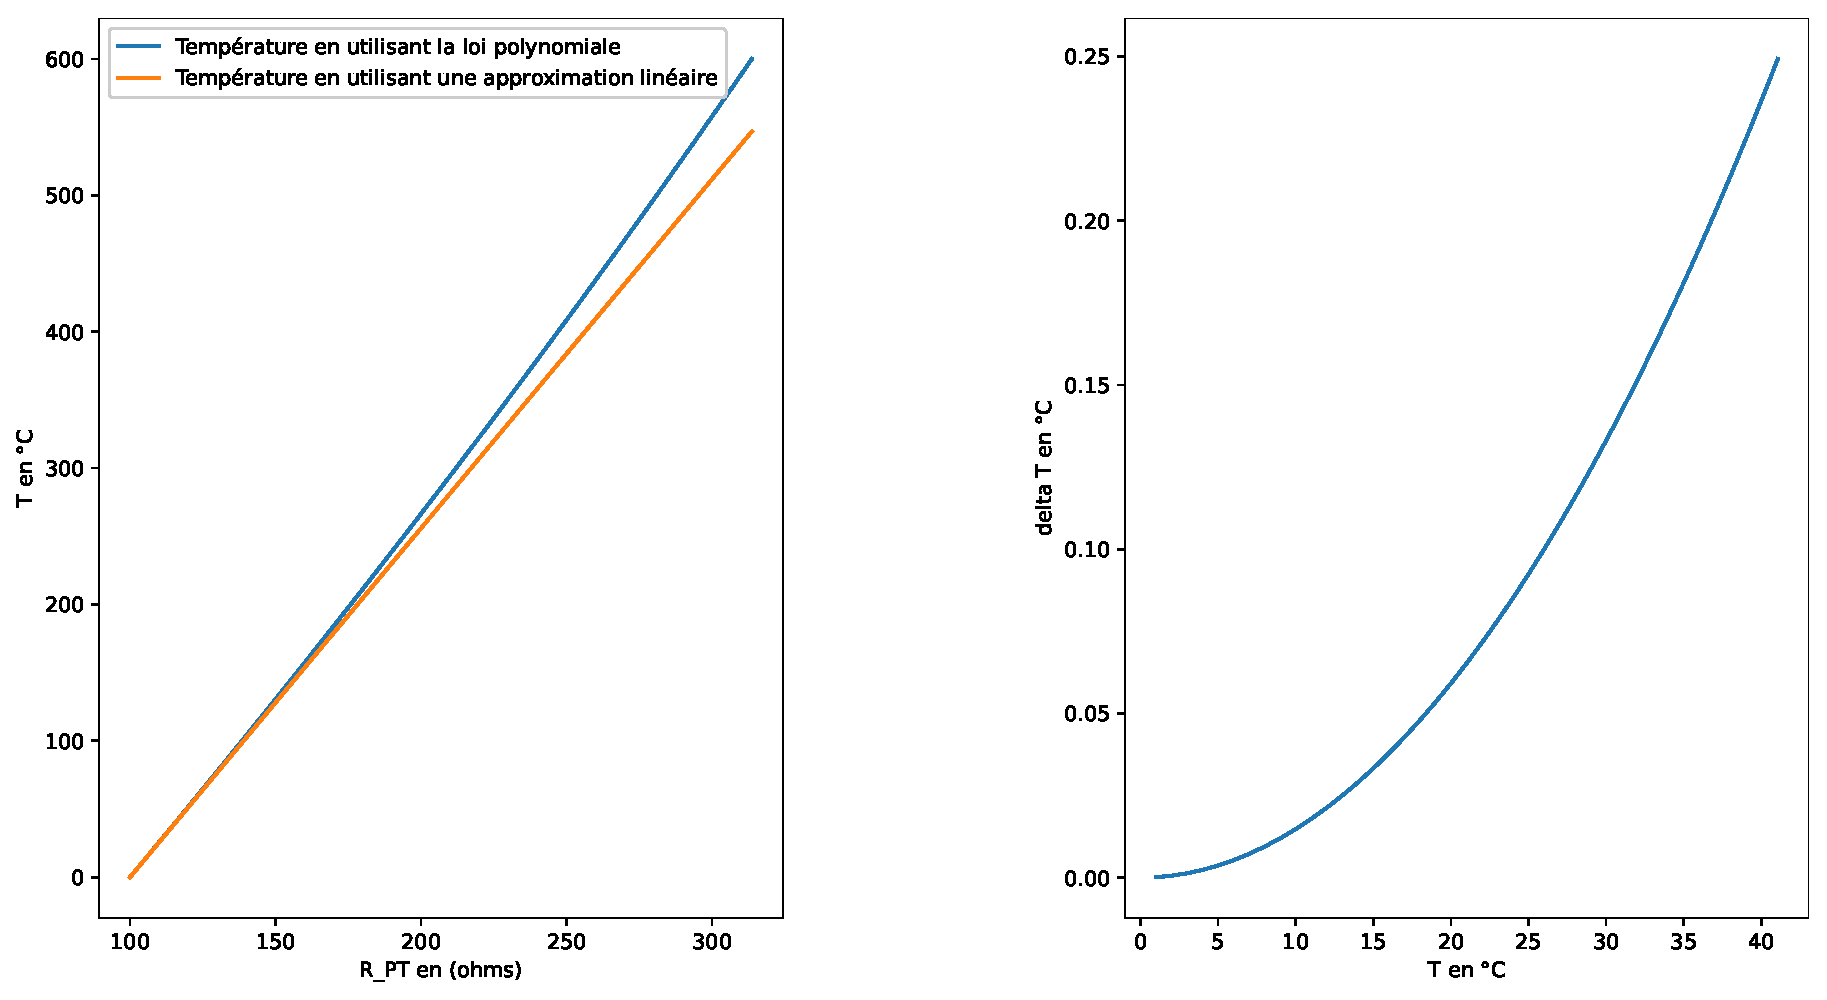
\includegraphics[scale=0.3]{Comparaison.eps}
		\label{Comparaison}
		\caption{Gauche: Comparaison des températures calculées avec les deux modèles. Droite: Différence entre les modèles pour des température ambiantes}
	\end{center}
\end{figure}

D'après l'équation (\ref{Modèle_linéaire}), on a donc la relation suivante:
\begin{equation}
T=\frac{R_{PT}-R_0}{a*R_0}
\label{Equation_température}
\end{equation}

En utilisant la formule du pont diviseur de tension, on trouve la relation entre $R_{PT}$ et $U_{PT}$:
\begin{align}
U_{PT}=\frac{R_{PT}}{R+R_{PT}}E \Rightarrow R_{PT}=\frac{R*U_{PT}}{E-U_{PT}}
\end{align}

\subsection{Mesures et expérimentation}



\end{document}
